%!TEX root = ../template.tex
%%%%%%%%%%%%%%%%%%%%%%%%%%%%%%%%%%%%%%%%%%%%%%%%%%%%%%%%%%%%%%%%%%%
%% chapter1.tex
%% NOVA thesis document file
%%
%% Chapter with introduction
%%%%%%%%%%%%%%%%%%%%%%%%%%%%%%%%%%%%%%%%%%%%%%%%%%%%%%%%%%%%%%%%%%%
\newcommand{\novathesis}{\emph{novathesis}}
\newcommand{\novathesisclass}{\texttt{novathesis.cls}}


%%-------------------------------------------------------------------
%%	1 - Introduction
%%-------------------------------------------------------------------
\chapter{Introduction}
\label{cha:introduction}

%\begin{quotation}
%  \itshape
%  This work is licensed under the Creative Commons Attribution-NonCommercial~4.0 International License.
%  To view a copy of this license, visit \url{http://creativecommons.org/licenses/by-nc/4.0/}.
%\end{quotation}


%%-------------------------------------------------------------------
%%	1.1 - Context
%%-------------------------------------------------------------------
\section{Context} % (fold)
\label{sec:intro_context}

The concept of virtualisation, despite all the recent discussion, isn’t new. In reality, this technology has been around since the 1960s~\cite{Buzen1973}, but it was not until the development of virtualisation technologies for the x86 architecture~\cite{Agesen2010} and the introduction of \textit{Intel VT}~\cite{Intel2010} and \textit{AMD SVM}~\cite{AMD2010} in the 2000s that virtualisation has entered the mainstream as the go-to technology solution for server deployment across many production environments. 

With efficient techniques that take advantage of all available resources, and a lowering price point on hardware, an opportunity for the advance of new application models and a revamp in the supporting infrastructure was generated. 

However, companies realised that the cost to run a fully fledged \textit{data centre} in-house is unreasonable and a cumbersome task. Not only taking into account the cost of the hardware, but factoring in the many requirements like the cooling systems that take care of the heat generated by the running machines, physical security to protect the rooms, fire suppressing systems in case of emergency, people to maintain the infrastructure, all added, result in considerable costs on a monthly basis.
Adding to this, the demand for instantaneous access to information and the extensive resources needed to store it does not stop growing.

This fact created an opening for a \gls{IaaS}~\cite{Mell2011} model, outsourcing all the responsibilities of storing the data and providing the needed computation resources from third parties, which are experts in maintaining huge data centres and even provide all this in various geographic regions.

With influential industry players following this trend, supporting more and more types of services and with an increasing number of customers joining this model, new ways to store the growing number of files have emerged. New file systems with a focus on reliability, consistency, performance, scalability, all in a distributed architecture are essential to a broad range of applications presenting a myriad of workloads.



%%-------------------------------------------------------------------
%%	1.2 - Motivation
%%-------------------------------------------------------------------
\section{Motivation} % (fold)
\label{sec:intro_motivation}

Virtualisation is the pillar technology that allowed for the widespread of the IaaS cloud providers in a model of economies of scale. These cloud providers, such as Amazon AWS~\cite{aws_2017}, Microsoft Azure~\cite{azure_2017} and Google Cloud Platform~\cite{gcp_2017}, manage thousands of physical machines all over the globe, with the majority of the infrastructure being multi-tenant oriented. 

The sheer magnitude of those numbers leads to an obvious problem. How to store all this data efficiently? Not only there is the need to store client generated data but also manage all the demands of the infrastructure and the many services offered. One approach taken by these companies was the development of their proprietary storage solutions. For instance, Google uses BigTable distributed storage system \cite{Chang2006}, to store product specific data, and then serve it to users. This system relies on the Google File System underneath to provide a robust solution to store logs and data files, designed to be reliable, scalable and fault tolerance.

One characteristic in particular that stands out and is present in many of today's systems is the use of snapshots with copy-on-write techniques. The adoption of such methods allows for quick copy operations of large data sets but saving resources. At the same time, it provides high-availability with read-only copies of the data always ready to use and allowing applications to continue execution of write operations simultaneously.
All the above-mentioned properties joined with others such as replication and data distribution, to comprise the fundamentals of what is needed to run a highly distributed and scalable file system. For instance, the duplication of records across multiple machines, not only serves as a security net in case of a misfortune event avoiding having a single point of failure but can also be used to maximise availability and take advantage of network bandwidth. 

%Existing file systems address some of these properties by default, however, in most cases, they were designed to be compatible with an increasing diversity of devices that run UNIX-based Operating Systems and need to offer a POSIX API, being more concerned with a local environment. 
%TODO
%\textbf{TO DO - Rephrase sentence above}\\

One of these newer systems that have a significant adoption by the Linux community is the BTRFS~\cite{Rodeh2013}. At the start, this file system already adopts an efficient system of snapshots, and it has as a primary design principle to maintain excellent performance in a comprehensive set of conditions.
The combination of this file system with replication and partitioning techniques opens the way to a solution that serves the needs of an up to date storage system, consequently having the possibility of being easily integrated into an existing platform, serving a vast number of clients and presenting outstanding performance. 



%%-------------------------------------------------------------------
%%	1.3 - Project Presentation
%%-------------------------------------------------------------------
\section{Project Presentation} % (fold)
\label{sec:intro_project_presentation}

This dissertation work is performed in the context of a more comprehensive project with the name \gls{iCBD}~\cite{Lopes2017}, under development at \textit{SolidNetworks – Business Consulting, Lda} part of the \textit{Reditus S.A.} group in collaboration with \textit{NOVA LINCS} hosted at \textit{DI - FCT/NOVA}.

The primary objective is to improve in a known model, the client-based Virtual Desktop Infrastructure, developing an infrastructure to support the execution, in a non-intrusive way, of virtualised desktops in conventional workstations.

%This dissertation work in enveloped in a larger project by the name iCBD, Infrastructure for Client-Based (Virtual) Desktop (Computing), were the objectives pass by the development of a computational infrastructure capable of supporting the execution of virtual desktops in an assortment of devices having as its main characteristic a non-intrusive approach. 

%Taking this into account, there is a clear separation from other solutions previously and currently available, where there is a concern for the target device, without any writing being done to the local disks, preserving all the stored data, and giving the possibility to have other operating systems available for a local boot. To achieve this objective, all the needed components are loaded on-demand at the system startup and as part of the boot.



%%-------------------------------------------------------------------
%%	1.3. - iCBD Project
%%-------------------------------------------------------------------
\subsection{iCBD Project} % (fold)
\label{sub:intro_icbd_project}

There are some leading-edge aspects of the \acrfull{iCBD} project which sets it apart from other existing solutions such as the adoption of a diskless paradigm with a remote boot, the way the platform stores \gls{VM} images, and the support for a virtualised or native execution on the target workstation~\footnote{In this document workstation is a user's desktop PC, laptop, etc., any PC compatible computing device.}, depending on the user's choice.~\cite{P2020}

The remote boot of the users workstation requires the cooperation of \acrshort{HTTP}, \acrshort{TFTP}, and \acrshort{DHCP} and image repository servers, that store VM templates as well as running instances based on them.
To address the process of communication between workstations and the platform it is used the HTTP protocol, providing flexibility and efficiency in the communication of the messages.~\cite{P2020,Nuno2016,Eduardo2016}

%\begin{figure}[htbp]
%    \centering
%    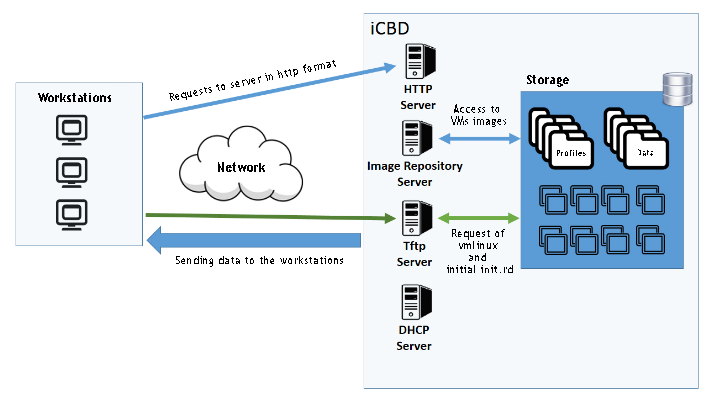
\includegraphics[height=3in]{cap1_icbd}
%    \caption{iCBD architecture. Adapted from \enquote{Linked clones baseados em funcionalidades de snapshot do sistema de ficheiros} by Nuno Alves~\cite{Nuno2016}}
%    \label{fig:icbd}
%\end{figure}

%\newpage

It is also interesting to briefly discuss some of the primary objectives of the project, being:
\begin{itemize}
    \item Offer a work environment and experience of use so close to the traditional one that there is no disruption for the users when they begin to use this platform.
    %
    \item Enable centralised management of the entire infrastructure including servers in their multiple roles, storage and network devices from a single point.
    %
    \item Complete decoupling between users and workstations in order to promote mobility.
    %
    \item Support the disconnected operation of mobile workstations.
\end{itemize}

With all the above in account, there is a clear separation from other solutions previously and currently available. As far as we know, no other solution is so comprehensive in the use of the resources offered by workstations whether they are PCs, laptops or similar devices.
\newpage


%%-------------------------------------------------------------------
%%	1.3. - Previous Work
%%-------------------------------------------------------------------
\subsection{Previous Work} % (fold)
\label{sub:intro_previous_work}

There have previously been two dissertations involved in this project. The work of those students has centred in the creation of the instances of virtual machines, more specifically in a creation supported by native snapshot mechanisms of the file system where the templates reside. Testing several Files Systems that present the requirements mentioned above. As well as, conduct an analysis on the performance of those systems when working with a typical load for the platform. 
In a few words, the work opens a path where the snapshots stop being tied to the hypervisor as a tool for the provisioning (thin or full) of clones and bestowing the job to the file system snapshot system, which is fundamental to deliver a centralised management solution.
As is happening presently, the two theses have followed two different paths in an attempt to determine which type of file system best suits these objectives. 
In that sense, one of the works was used a local file system, named BTRFS, as the other followed the object-based storage path, adopting the CephFS.



%%-------------------------------------------------------------------
%%	1.4 - Problem Stating and Main Contributions
%%-------------------------------------------------------------------
%\section{Problem Stating and Main Contributions} % (fold)
\section{Problem Stating and Main Contributions}
\label{sec:intro_project_contributions}

This dissertation aims to build upon the previous contributions, deeply study the core of the iCBD platform and tackle the next set of questions, mainly:

\begin{itemize}
	%\item \textit{Needing a distribute data model between nodes, which can be set apart geographically, how to achieve that and maintain the consistency and availability of the data?}
	%\item \textit{How to scale the platform in order to handle a large number of clients and maintain or even enhance the performance?}
	\item \textit{In a geographically dispersed, multi-server iCBD infrastructure, how do we keep the VM templates consistent and available even on the presence of network faults?}
	%
	\item \textit{How do we keep the management of templates across multiple "zones", simple?}
	%
	\item \textit{How to scale the platform in order to handle a large number of clients and maintain or even enhance its performance?}
\end{itemize}




%%-------------------------------------------------------------------
%%	3.2. - Replication and Caching - The Problem 
%%-------------------------------------------------------------------
\subsection{Replication and Caching - The Problem}
\label{sec:intro_replication_cache_theproblem}

To answer these questions, we can formulate small topics that guide the work in a more focused way creating a list of general requirements to be addressed by this thesis.
In general, the work will be divided into two major subjects, were the second is a direct consequence and requires the first.


%\subsection{Motivation and Goals}
\paragraph{Motivation and Goals}
\label{par:intro_motivation_goals}

Providing a mechanism that ensures the correct replication of data between nodes of the platform is paramount. This process also needs to confer other properties such as achieving the best performance on data transferences, being in a factor of speed or the used bandwidth. Another point of interest is the fact that the replication process should easily integrate with any File System used in the Storage Layer (taking into account that is fundamental that the file system provides some variety of snapshotting mechanism) trying not to add a sizeable computational load.
Following this idea, we may start thinking on how to deliver to the clients the benefits of replicating data. The replication procedure is not only a useful tool to propagate efficiently data changes throwout the nodes of the platform and act as insurance from a data loss disaster, but also capitalise on getting closer to the clients the resources that they need. Following this line of thought, an answer to the second question starts to appear. It is not only necessary to think about the location of the data, but also to study which services are used by the platform that are fundamental for running images on the client's workstations and how to integrate all so as to deliver the best experience to the highest number of clients.
To summarise, the following list poses the key requirements had in mind during the planning and execution of this effort:

\begin{itemize}
    \item The iCBD platform needs to be always available and maintain top-notch performance in multiple locations while serving a considerable number of clients.
    %
    \item Produce a mechanism that allows the replication of data not only for security reasons (backup) but also providing that data closer to the client.
    %
    \item With the data near its consumer study what is required to deliver that data to the client in the most efficient way.
	%
	\item Boot a client with the minimal number of the platform functionalities possible, simplifying the processes near the consumer.
\end{itemize}

%\subsection{System Overview}
%\label{sub:system_overview}

%\subsection{Requirements}
%\label{sub:requirements}



%%-------------------------------------------------------------------
%%	1.3. - Main Expected Contributions
%%-------------------------------------------------------------------
\subsection{Main Expected Contributions} % (fold)
\label{sub:intro_main_expected_contributions}

The main expected contributions are: 

\begin{itemize}
  \item Perform a throughout analysis of the already implemented iCBD platform modules and the several layers where it expands in order to understand the inner works, providing an excellent platform to build upon and allowing for an efficient planning of the remaining work. 
  %
  \item The study, develop, and evaluate an implementation of a distributed and replicated BTRFS file system for VM storage.
  %
  \item Implement a client-side caching solution in order to increase availability, improve response time, and enable better management of resources.
  %
  \item Integrate the solutions described above  with the work previously developed and the existing infrastructure
  %
  \item And finally, carry out a series of tests that lead to a meaningful conclusion and that provide help in the design of the remaining platform.
\end{itemize}


In a more concrete approach, we present the work plan, for achieving the above objectives, distributed by the two main topics.


%\subsubsection{Replication}
\paragraph{Replication}
\label{par:intro_replication_goals}

\begin{itemize}
	\item Create a middleware that integrates with the core functionalities already developed within the iCBD platform.
	%
	\item Should aim to be storage provider agnostic (in this thesis work with BTRFS but remain easy to integrate with others).
	%
	\item Work with compression algorithms to achieve a lower bandwidth consumption.
	%
	\item Be able to use encrypted and unencrypted communications for all data flows. 
	%
	\item Capitalize the snapshotting features of the storage layer in order to minimise the volume of data transferred, only sending the differences between versions whenever possible.
	%
	\item Provide a simple CLI and a REST API for interacting with the replication module functions.
\end{itemize}

This subject is further developed in \textbf{Section~\ref{sec:impl_icbdrep}}.

%\subsubsection{Cache Server}
\paragraph{Caching}
\label{par:intro_caching_goals}

\begin{itemize}
	\item Dilute some cost of the infrastructure by having commodity hardware as proximity servers.
	%
	\item Bring the data closer to the final clients giving enough storage capacity to servers, storing the most used images.
	%
	\item Facilitate a user experience where the is no distinction on booting an OS from a local disk or the iCBD platform.
	%
	\item Build a completing working iCBD platform on the FCT NOVA campus.
	%
	\item Study the benefits of introducing cache servers and the platform performance as a whole, comparing the performance of the system to a traditional OS install base.  
\end{itemize}

A detailed view of this work is presented in \textbf{Section~\ref{sec:impl_cache_server}}.
% subsection main_expected_contributions (end)



%%-------------------------------------------------------------------
%%	1.5 - Document Structure
%%-------------------------------------------------------------------
\section{Document Structure} % (fold)
\label{sec:intro_document_structure}

The remnant document is structured as follows: 

\begin{itemize}

  \item \textit{Chapter~\ref{cha:research_context}}  \textbf{Research Context} - This section presents existing technologies and theoretical approaches which were the target of study, such as, storage systems and several of its features, as well as several intrinsic characteristics of virtualisation techniques.
	%
  \item \textit{Chapter~\ref{cha:icbd}} \textbf{iCBD - Infrastructure for Client-Based Desktop} - In this chapter, there is a presentation of the iCBD platform as a whole. Giving also an overview of the solution with its multiple layers and trying to explain the conceptual and architectural decisions made, being essential to understanding the bigger picture and where the remaining work fits in.
  %
  \item \textit{Chapter~\ref{cha:impl_replication_caching}} \textbf{Implementation of the \textit{iCBD-Replication and Cache Server}} - Starts giving an in-depth view of the implementation of the iCBD Replication module, detailing the architectural decisions and the implemented components. Then, follows a description on the efforts to build a test infrastructure on the FCT NOVA grounds, solely dedicated to the iCBD project. Concluding the chapter with an explanation on how to build and deploy an iCBD Cache Server node that can serve the entirety of workstations on a laboratory in the Computer Science Department.
  %
  \item \textit{Chapter~\ref{cha:evaluation}} \textbf{Evaluation} - The evaluation process employed in the validation of our implementation is presented in this chapter. Emphasizing the results of the work developed, analysing the results obtained and comparing with baseline values.
  %
  \item \textit{Chapter~\ref{cha:conclusion}} \textbf{Conclusions \& Future Work} - This last chapter concludes the dissertation by answering the questions stated in the Introduction, summarising the results achieved in the evaluation process and presents some improvements ideas that wore formulated during the implementation process and are believed to be a good starting point for future work.
\end{itemize}

% section document_structure (end)
